\documentclass[12pt]{article}
\usepackage[utf8]{inputenc}
\usepackage{listings}
\usepackage{color}
\usepackage{hyperref}
\usepackage{natbib}
\usepackage{graphicx}
\usepackage{xparse}
\usepackage{amsmath}
\usepackage{amssymb}
\usepackage{mathtools}
\usepackage[font=small,labelfont=bf]{caption}
\title{Bachelor Thesis\\ Decoding the Color Code}
\author{Clemens Schumann, \\
Advised by Peter-Jan Derks}

\begin{document}
\maketitle
\newpage
\tableofcontents
\newpage
%\section{Abstract}
%In this thesis I will propose a color code decoding algorithm
and provide an implementation of it.

\section{Overview of QEC algebra}
A quantum computer operates on so-called $qudits$, which can be
any multi-level quantum system. 
Physical implementations of these include particles with 
spin, as well as controlled EM-waves, i.e. lasers. \\
In this thesis we will
focus on \emph{qubit}-based systems, i.e. two-level quantum systems as base 
units of computation.

In the following we will analyze quantum circuit diagrams using the different
pictures of quantum mechanics.
A quantum circuit diagram is a visual representation of the computation done
in a quantum computer, whereby:
\begin{itemize}
	\item States progress in time along horizontal parallel lines
	\item Time goes from left to right
	\item Gates denoted X,Y,Z are the single qubit pauli operators
		$\sigma_x,\sigma_y,\sigma_z$
	\item Gates can act on one or multiple qubits, whereby an X gate 
		on qubit 1 in a 3-qubit system should be interpreted as:
		\\$(X\otimes \mathbb{I} \otimes \mathbb{I}) (|\psi_1\rangle
		\otimes |\psi_2\rangle \otimes |\psi_3\rangle)$
\end{itemize}
\begin{figure}[h!]
	\begin{center}
	\captionsetup{justification=centering,margin=2cm}
	\includegraphics[scale=0.4]{img/cnotMeasureCircuit.png}\\
	\caption{A Quantum Circuit to implement a measurement based\\
		Controlled-$X_{|\psi\rangle_{control}\rightarrow |\psi\rangle_{target}}$ Gate,
		where $|0\rangle$ is the +1 eigenstate in $\sigma_{z}$-basis.}
	\label{fig:circuit1}
	\end{center}
\end{figure}
\subsection{Schroedinger picture}
In the Schroedinger picture, we focus on the time evolution of qubit states:
\begin{equation}  
	|\psi\rangle = |\psi(t)\rangle 
\end{equation}

Measurements project these states onto eigenstates of the measurement operators via
a projection $P$, so:

\begin{equation}
    P_M^{\pm} |\psi\rangle = \frac{(M\pm \mathbb{I})|\psi\rangle}{2}
\end{equation}
Where $M$ is a matrix representation of the physical observable
 to be measured.
For example, a measurement of a single qubit's spin along the z-axis would be
represented as:
\begin{equation}
    M_Z = \left(
        \begin{array}{cc}
            1 & 0 \\
            0 & -1 \\
        \end{array}
        \right)
\end{equation}
And that measurement would perform a projection $P_Z$:
\begin{equation}
    P_Z^+ = \left(
        \begin{array}{cc}
            1 & 0 \\
            0 & 0 \\
        \end{array}
        \right)
    or
    P_Z^- = \left(
        \begin{array}{cc}
            0 & 0 \\
            0 & 1 \\
        \end{array}
        \right)
\end{equation}
on the state, depending on whether the measurement result yielded $+1$ or $-1$.

Therefore, to calculate the output of a quantum circuit in the Schroedinger
picture, simply apply the measurements and gates on the input states.
\begin{figure}[h!]
	\begin{center}
	\captionsetup{justification=centering,margin=2cm}
	\includegraphics[scale=0.4]{img/figures/cnotMeasureCircuit.png}\\
	\caption{A Quantum Circuit to implement a measurement based\\
		Controlled-$X_{|\psi\rangle_{control}\rightarrow |\psi\rangle_{target}}$ Gate,
		where $|0\rangle$ is the +1 eigenstate in $\sigma_{z}$-basis.}
	\label{fig:circuit1}
	\end{center}
\end{figure}
As can be seen explicitly calculated in the Schroedinger 
picture in Appendix~\ref{sec:calc1}, the circuit from Figure~\ref{fig:circuit1}
implements a CNOT gate from the control qubit to the target qubit.

We will now analyze this circuit in the Heisenberg picture\cite{gottesman},
finding that it results in an equal output.

\subsection{Heisenberg picture and stabilizer formalism}
\subsubsection{Stabilizer group}
We call an operator/gate S, to which the input state is an
eigenvector ($S|\psi\rangle=|\psi\rangle$), a $stabilizer$ of that input state. 
For $n$-qubit systems, we write these stabilizers as $n$-tensor-products 
of pauli operators $P \in P_{G}$,
where $P_{G}$ is the group generated by the Pauli operators and
the Pauli operators are the operators on $\mathbb{F}_{2}$ such that:

\begin{equation}
    \forall P\in P_{G}: P^{2}=\mathbb{I}.
\end{equation}

In the Heisenberg picture, stabilizers are tracked instead of
states. 
The stabilizer group $S_{G}$ is the group generated by
the set of stabilizers:
\begin{equation}
	S_{G} = \langle S_{0},..,S_{n}\rangle: S|\psi_{in}\rangle = 
	|\psi_{in}\rangle \forall S \in S_{G}
\end{equation}

So for the example in Figure~\ref{fig:circuit1} it is the group
of operators to whom
$|\psi_{control}\rangle \otimes |0\rangle \otimes 
|\psi_{target}\rangle$ is an eigenstate, namely 
$\mathbb{I}\otimes Z \otimes \mathbb{I}$ (and trivially
$\mathbb{I}\otimes\mathbb{I}\otimes\mathbb{I}$, which we choose
to ignore as a stabilizer since any three-qubit state
is stabilized by it, and it can be generated by squaring any
stabilizer constructed through tensor products of Pauli matrices).

A stabilizer group is always an abelian group i.e. its elements 
 commute, since if:

\begin{equation}
	\label{abelian_stabilizers_equation}
	\forall A,B \in S: AB|\psi\rangle = BA|\psi\rangle = |\psi\rangle
	\Rightarrow [A,B]|\psi\rangle=0
\end{equation}

\subsubsection{Effect of gates on stabilizers}
To determine the effect a gate operation A has on a
stabilizer, consider the following:

If $S|\psi\rangle = |\psi\rangle$ then:
\begin{equation}
A|\psi\rangle = AS|\psi\rangle = AS\mathbb{I}|\psi\rangle
	= \underbrace{ASA^{\dagger}}_{=S'}A|\psi\rangle
\end{equation}
So we now know that the post-gate state is an eigenstate of $S'$.

Therefore $S'_{G} = \langle AS_{0}A^{\dagger},...,AS_{n}A^{\dagger}\rangle$.


\subsubsection{Effect of measurements on stabilizers}
After a measurement $M$, an $n$ qubit input state will always 
collapse into either the +1 or the -1 eigenstate of the 
measurement operator.
In the first case the acting measurement operator was 
$\mathbb{I}^{\otimes n}+M$, in the second it was
$\mathbb{I}^{\otimes n}-M$.

A Pauli measurement operator $M$ can either commute with all stabilizer
operators, in which case $M$ itself is a stabilizer already. In this case
the measurement has no effect on the state, since the measurement of a
stabilizer projects onto identity.
Otherwise it can anticommute with at
least one operator in $S_{G}$, since Pauli operators as well as
their tensor products can only commute or anti-commute with each
other. The product of two operators that both anticommute with another operator
will then commute with that operator.

So in order to obtain the new stabilizers  $S'_{G}$:
\begin{enumerate}
	\item Identify $S\in S_{G}: \{S,M\}=0$
	\item Remove S from $S_G$
	\item Add $M$ to $S_G$ 
	\item replace each $N \in S_G \cup\overline{X}\cup\overline{Z}$
		with SN if $\{N,M\}=0$
\end{enumerate}
where $\overline{X}$ and $\overline{Z}$ are the sets of 
logical X and Z operators respectively. A logical operator is
an operator which acts on a systems metastructure that can be treated
as its own qubit.

\subsubsection{Circuit Analysis in Stabilizer formalism}

In the following, stabilizers
will be written without the tensor product symbols, so in 
our case the stabilizer is initially: $S_{G}^{0}= \langle IZI \rangle$,
the logical $\overline{X}$ operator is XXX and the logical
$\overline{Z}$ operator is ZIZ.

 In the circuit shown in 
Figure~\ref{fig:circuit1}, the measurements project onto:

\begin{align}
	P^{\pm}_{1} &= \frac{1}{2}\left(\mathbb{I}^{\otimes 3} \pm 
	\mathbb{I}\otimes X \otimes X\right) \\
	P^{\pm}_{2} & = \frac{1}{2} \left(\mathbb{I}^{\otimes 3} \pm
	X \otimes X \otimes \mathbb{I}\right) \\
	P^{\pm}_{3} &= \frac{1}{2} \left(\mathbb{I}^{\otimes 3} \pm
	\mathbb{I} \otimes X \otimes \mathbb{I}\right)
\end{align}

After the first measurement, the state is stabilized by 
IXX, since it collapses into an eigenstate of the measurement 
operator. Notably, if the measurement operator M anticommutes
with some element of the stabilizer S:

\begin{equation}
	SP_{-}S^{\dagger} = \frac{1}{2}S\left( 
	\mathbb{I}^{\otimes 3} - M \right) S^{\dagger}
	= \frac{1}{2} \left( \mathbb{I}^{\otimes 3} + M \right)
	SS^{\dagger} = P_{+}
\end{equation}

So by applying an anticommuting previous stabilizer operator
after the measurement one can ensure that the state is in the
$P_{+}$ projected state $P_{+}|\psi_{init}\rangle$ (in short,
+1 and -1 eigenstates have the same stabilizers if we add 
conditional gates accordingly).

% For the logical operators, if $\overline{X}$ or $\overline{Z}$
% do not commute with the measurement operator, we know that their
% product with another anticommuting operator from the previous
% stabilizer must then commute with the measurement operator: 
% $[S_{prev}\overline{X}M, MS_{prev}\overline{X}]=0$ (recall the
% previous statement that all Paulis and their tensor products must
% either commute or anti-commute).

In our case, IZI and IXX anticommute,
so now the state is stabilized by $S^{1}_{G} = \langle IXX
\rangle$. Both initial logical operators commute with the first
measurement operator, so they are left unchanged.

After the second measurement $M_{2}$=ZZI, since this
measurement anticommutes with the IXX stabilizer, the new 
stabilizers are: $S^{2}_{G}=\langle ZZI \rangle$. The logical 
$\overline{X}$ and $\overline{Z}$ operators are unaffected
, since they commute with the measurement operator.

After the third measurement $M_{3}$ =IXI, since this measurement
anticommutes with the stabilizer, the new stabilizers are:
$S^{3}_{G}= \langle IXI \rangle$. The logical $\overline{Z}$
operator anticommutes with the measurement, so is replaced by\\
$ \overline{Z_{3}} $=ZZI $\cdot$ ZIZ = IIZ\@. The logical 
$ \overline{X} $ is unaffected since it commutes with the
measurement operator. 

The stabilizer for the control and target qubit is still
identity, and logical $\overline{Z}: ZIZ \rightarrow IIZ$.

Since this circuit maps $Z_{control}\otimes Z_{target} \mapsto I_{control}
 \otimes Z_{target}$,
and via a similar analysis it can be shown that it also maps
$I\otimes Z \mapsto Z \otimes Z$, $Z\otimes I \mapsto Z \otimes I$,
$X\otimes I \mapsto X \otimes X$ and $I\otimes X \mapsto I \otimes X$,
this circuit implements a logical CNOT from the first to the third qubit.

\newpage
In classical computation, a \emph{complete logical signature} is a group of
operators, which can be successively applied to express any general boolean 
computation. One example of such a signature is $\{\neg, \land\}$. 
A quantum equivalent of this is the Pauli Group amended by the 
\emph{Clifford group}, 
whereby the Clifford group is the group of operators that project eigenstates
of a Pauli group operator onto an eigenstate of a Pauli group operator.

While not enabling universal computation (e.g. the phase 
estimation in Shor's algorithm \cite{shor} would require an additional T gate),
the union of Clifford and Pauli group \emph{is} a complete logical signature for those quantum
operations that can be simulated efficiently on a classical computer
\cite{gottesmanFaultTolerant}.
This is relevant for quantum error correction, as applying corrective gates after
an error is computationally and experimentally expensive and should therefore be put
off until the first non-Clifford gate is encountered in the program. Until that 
point the propagation of the error through the circuit can be simulated
efficiently.

The Clifford Group can be generated by:

\begin{itemize}
    \item The Hadamard-Gate $H$, which performs single qubit
    basis changes from eigenstates of X to eigenstates of Z 
    and vice-versa:

    $H|+\rangle = |0\rangle$, $H|0\rangle = |+\rangle$,
    $H|-\rangle = |1\rangle$, $H|1\rangle = |-\rangle$
    
    \item The Phase-Gate $P$, which performs single qubit sign
    flips on the state parts which are $|1\rangle$ in the 
    computational basis:

    $
    P (\alpha|0\rangle \pm \beta |1\rangle) =
    \alpha|0\rangle \mp \beta |1\rangle
    $

    \item The CNOT-Gate, which on a two qubit system performs 
    an X gate on the second qubit if the first qubit is 
    $|1\rangle$, so maps:

    $
    \alpha |00\rangle + \beta |01\rangle + 
    \delta |10\rangle + \gamma |11\rangle \\
    \mapsto
    \alpha |00\rangle + \beta |01\rangle +
    \gamma |10\rangle + \delta |11\rangle
    $
\end{itemize}
In the $\sigma_z$-basis their matrix representations are:
\begin{itemize}
    \item
    \begin{math}
    H = 
    \frac{1}{\sqrt{2}}\cdot\left( 
    \begin{array}{cc}
       1 & 1 \\
       1 & -1 \\
    \end{array}
    \right)\end{math} 
;
    \begin{math}
    P = 
    \left(\begin{array}{cc}
        1 & 0 \\
        0 & i \\
    \end{array}\right)
    \end{math}
    
    \item 
    \begin{math}
    CNOT = 
    \left(\begin{array}{cccc}
        1 & 0 & 0 & 0 \\
        0 & 1 & 0 & 0 \\
        0 & 0 & 0 & 1 \\
        0 & 0 & 1 & 0 \\
    \end{array}\right)
   \end{math} 
\end{itemize}

\newpage
\section{Error detection and correction}

\subsection{Quantum Error Model}
This way of encoding information however leaves a notable
issue:

It only detects bitflip, or Pauli-X, errors occurring on
the stored quantum information. While using Hadamard gates one
could trivially adapt this code to instead detect Pauli-Z errors,
it is not possible to use linear codes like the repetition code
to $simultaneously$ detect Pauli-X and Pauli-Z errors occurring.

Unlike classical computers, on a quantum computer the type of error
 is not limited
to a bitflip. Even single qubit states have an
infinite amount of differing states to it, since when representing a single
qubit state as a vector on a Bloch sphere it immediately becomes apparent
that there are an infinite number of vectors on that sphere which are different
from it. It turns out though, that the change in state from one normalized
one to another is merely a sum of two rotations.

Fortunately, noise can therefore be modeled as a sum of Pauli gates.
Any single qubit error operator matrix E can be written as:
\begin{equation}
    E =
    \left(
    \begin{array}{cc}
        a & b \\
        c & d \\
    \end{array}
    \right) = 
    \alpha \mathbb{I} + \beta X + \delta Y + \gamma Z
\end{equation}
With an apropriate choice of $\alpha, \beta, \gamma, \delta$.
In effect, this means that with probability $\alpha$, the effect of the
error $E|\psi\rangle$ will be $\mathbb{I}$; with probability $\beta$ its effect
will be X, and so on.

It is hence sufficient to determine which of these errors $\mathbb{I}$, 
X, Y or Z has occurred, and we can apply the same operator again to return to the 
initial state.
Since an identity noise occurring is irrelevant to us, and XY as
well as ZY (anti-) commute, we need only detect for X and Z
errors occurring in order to detect any single qubit errors. 

\subsection{Classical/ Linear codes}
From classical computer science there are well known existing
encoding schemes, such as the repetition and ring code.
We call these codes linear because their graph representations are
linear, or one-dimensional. In Quantum error correction, we speak of $[[n,k,d]]$ stabilizer
codes if an encoding scheme allows for $n$ physical qubits to 
encode $k$ logical qubits to an error distance of $d$, i.e. $d$ individual errors 
being corrigible.
In the following I will refer to linear or classical codes as having a 
distance of $\frac{1}{2}$, to indicate that they do not protect against an
arbitrary single qubit error, but only against flips in one specific eigenbasis.
\subsubsection{Repetition code}
For this error code information is encoded by repeating the 
intended message some amount of times, and then decoding it
by performing a majority vote on the transmitted message.


\begin{figure}[h!]
	\begin{center}
	\captionsetup{justification=centering,margin=2cm}
	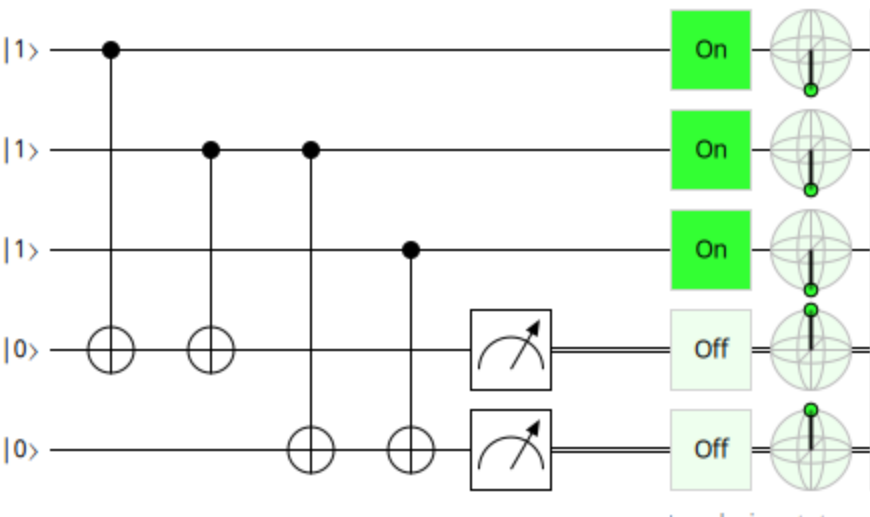
\includegraphics[scale=0.2]{./img/bitflipSyndromeExtraction3Rep.png}\\
	\caption{Bitflip Syndrome extractor\\
        +1 measurement result on first Ancilla indicates a bitflip error
        on qubits 1 or 2, +1 result on second ancilla indicates 
		bitflip on second or third qubit}
	\label{fig: syndrome extractor}
	\end{center}
\end{figure}

A quantum equivalent of the 3-bit repetition code performed on
the message $|1\rangle$ is is the [[3,1,$\frac{1}{2}$]] repetition
code depicted in 
figure~\ref{fig: syndrome extractor}, including so-called
$syndrome\ extraction$. A syndrome is a stabilizer that can be
measured to detect whether and where an error has occurred
in a multi-qubit system. It is crucial that the 
measurement of such syndromes occurs without harming the actual
quantum information stored in the $data-qubits$. Therefore
two additional $ancilla-qubits$ (both initialized to 
$|0\rangle$) are attached to the circuit via CNOTs.
This circuit is stabilized by IZZ and ZZI, measured by ancilla 
1/2. The measurement result will therefore be a vector of length
two, with each entry either being +1 or -1. To simplify the 
algebra this will be changed to the binary representation of 0 
for +1 and 1 for -1. 

To represent the code, Stabilizers can be stacked together to
a so-called parity-check-matrix, which satisfies:
\begin{equation}
	M_{pc}\cdot \vec{v}_{error} = \vec{v}_{syndrome}
\end{equation}
So e.g. the parity check matrix for the $[3,1,\frac{1}{2}]$
repetition code would be:

\begin{equation}
	M_{pc3} = \left( 
	\begin{array}{ccc}
		1 & 1 & 0 \\
		0 & 1 & 1
	\end{array}
	\right)
\end{equation}
And the syndrome for an X error on the first qubit would be
$\left(\begin{array}{c}1\\0\end{array}\right)$.

This way of encoding information however leaves two notable
issues:

For one, it only detects bitflip, or Pauli-X errors occuring on
the stored quantum information. While using Hadamard gates one
could trivially adapt this code to instead detect Pauli-Z errors,
it is not possible to use linear codes like the repetition code
to $simultaneously$ detect Pauli-X and Pauli-Z errors occurring.

Secondly, it also assumes a noise model of a ``Noisy Channel'',
which is not compatible with the actually encountered errors in
real physical quantum computers.
\subsubsection{Ringcode}
The ring code's graph essentially just loops aroung at the repetition
code's single-edged nodes, so for example its edge matrix or parity-check
matrix for a three-qubit system looks like:
\begin{equation}
    M_{pc3} = \left(
        \begin{array}{ccc}
            1 & 1 & 0\\
            0 & 1 & 1\\
            1 & 0 & 1\\
        \end{array}
        \right)
\end{equation}
INSERT FIGURE SHOWING RINGCODE
\newpage
\subsection{2D codes}
Previous research in computer science 
provides a toolset for generating valid codes
from existing encoding schemes. 
Hypergraph product codes, introduced by Tillich and Z\'emor,
of two 
existing codes will always remain a valid detection code.

The parity check matrix $H$ of a hypergraph product code is generated
by the parity check matrices of two valid codes in the following
way:
\begin{equation}
	H = \left(\begin{array}{cc}
		M_{pcX} & 0 \\
		0 & M_{pcZ} \\
	\end{array}\right)
\end{equation}

\subsubsection{Surface code}
We can therefore form a hypergraph product code of two repetition
codes for X error detection and Z error detection respectively,
obtaining the [[$d^2$,1,d]]``Surface-Code'' which can detect up
to d of $both$ X and Z errors, and 
therefore any pauli error happening.
We can draw this code as a graph, whereby the code's stabilizers
are understood as an adjacency Matrix, the data qubits are on 
edges of the graph and the ancilla qubits for Z-checks are on faces
while the ancilla qubits for X-checks lie on nodes.\\
Like the repetition code, the Surface code is a code that is regular until
it's boundary nodes.

INSERT FIGURE SHOWING TORIC CODE

\subsubsection{Toric code}
Similarly, a hypergraph product code of two ring codes can be 
generated. We call this code the "Toric code".\\
INSERT FIGURE SHOWING TORIC CODE

\subsubsection{Color code}
\newpage
\subsection{Decoding schemes}

\section{Conclusion}
In this thesis, we gave an overview of existing
quantum codes as well as some decoding schemes.
The determined thresholds of ca. 16\% for the surface/toric code were
within the literature expected range(ADD REFERENCE). 
Their thresholds were however not distinguishable, and
especially for the cylindric code in future works, it might be of interest to 
calculate these thresholds more precisely by using more significant computational
resources.
The pseudo-threshold for the Steane code was found to be around $10^{-5}$, which is
the same as in the literature\cite{steaneThreshold}. 
While the lifting decoder for the hexagonal toric lattice color code did not produce
thresholdable output, it did work as a proof-of-concept on smaller error vectors as in
\ref{fig: lifting}.
Future work could include adapting a better cycle-finder algorithm for the lifted 
subgraph.
\newpage
\section{Appendix}
\subsection{Schroedinger picture calculation of CNOT circuit}
\label{sec:calc1}

In the quantum circuit depicted in figure \ref{fig:circuit1} the input
state can be written as $|\psi_{control}\rangle \otimes |0\rangle 
\otimes |\psi_{target}\rangle$ and the measurement in the first 
timestep can be expressed as $\mathbb{I}\otimes X \otimes X$.\\
\\
The initial state $|\phi_{t=0}\rangle$ = $|\psi_{control}\rangle \otimes |\psi_{ancilla}\rangle \otimes
|\psi_{target}\rangle$\\
where\\
$|\psi_{control}\rangle = \alpha|0\rangle+\beta|1\rangle$
\\
$|\psi_{ancilla}\rangle = |0\rangle$
\\
$|\psi_{target}\rangle = \gamma|0\rangle+\delta|1\rangle$
\\
therefore:
\begin{equation}
|\phi_{t=0}\rangle = \alpha \left( \gamma |000\rangle + \delta |001\rangle\right)+
\beta \left( \gamma |100\rangle + \delta |101\rangle \right)
\end{equation}

If the first measurement result is +1, the state becomes:
\begin{align*}
	|\phi^{+}_{t=1}\rangle 
	&= \frac{1}{2}\left(\mathbb{I}\otimes\mathbb{I}\otimes\mathbb{I}+
	\mathbb{I}\otimes X \otimes X\right)|\phi_{t=0}\rangle\\
	&= \alpha \left( 
	\gamma \left( |000\rangle + |011\rangle \right) +
	\delta \left( |001\rangle + |010\rangle \right) \right) \\
	&+ \beta \left(
	\gamma \left( |100\rangle + |111\rangle \right) +
	\delta \left( |101\rangle + |110\rangle \right) \right)
\end{align*}
if the result is -1, it becomes:
\begin{align*}
	|\phi^{-}_{t=1}\rangle 
	&= \frac{1}{2}\left(\mathbb{I}\otimes\mathbb{I}\otimes\mathbb{I}-
	\mathbb{I}\otimes X \otimes X\right)|\phi_{t=0}\rangle\\
	&= \alpha \left( 
	\gamma \left( |000\rangle - |011\rangle \right) +
	\delta \left( |001\rangle - |010\rangle \right) \right) \\
	&+ \beta \left(
	\gamma \left( |100\rangle - |111\rangle \right) +
	\delta \left( |101\rangle - |110\rangle \right) \right)
\end{align*}

In the case of the +1 Measurement $\rightarrow$ a=0:
\begin{align*}
	|\phi^{++}_{t=2}\rangle 
	&= \frac{1}{2}\left(\mathbb{I}\otimes\mathbb{I}\otimes\mathbb{I}+
	Z\otimes Z \otimes \mathbb{I}\right)|\phi^{+}_{t=1}\rangle\\
	&= (|000\rangle\langle000| +|001\rangle\langle001| +
	|110\rangle\langle110| +|111\rangle\langle111|)|\phi^{+}_{t=1}\rangle\\
	&= \alpha \left( \gamma |000\rangle + \delta |001\rangle \right)
	+ \beta \left( \gamma |111\rangle + \delta |110\rangle\right) 
\end{align*}
\begin{align*}
	|\phi^{+-}_{t=2}\rangle 
	&= \frac{1}{2}\left(\mathbb{I}\otimes\mathbb{I}\otimes\mathbb{I}-
	Z \otimes Z \otimes \mathbb{I}\right)|\phi^{+}_{t=1}\rangle\\
	&= (|010\rangle\langle010| +|011\rangle\langle011| +
	|100\rangle\langle100| +|101\rangle\langle101|)|\phi^{+}_{t=1}\rangle\\
	&= \alpha \left( \gamma |011\rangle + \delta |010\rangle \right)
	+ \beta \left( \gamma |100\rangle + \delta |101\rangle \right) 
\end{align*}
In the case of the -1 Measurement $\rightarrow$ a=1:
\begin{align*}
	|\phi^{-+}_{t=2}\rangle 
	&= \frac{1}{2}\left(\mathbb{I}\otimes\mathbb{I}\otimes\mathbb{I}+
	Z\otimes Z \otimes \mathbb{I}\right)|\phi^{-}_{t=1}\rangle\\
	&= \alpha \left( \gamma |000\rangle + \delta |001\rangle \right)
	- \beta \left( \gamma |111\rangle + \delta |110\rangle\right) 
\end{align*}
\begin{align*}
	|\phi^{--}_{t=2}\rangle 
	&= \frac{1}{2}\left(\mathbb{I}\otimes\mathbb{I}\otimes\mathbb{I}-
	Z\otimes Z \otimes \mathbb{I}\right)|\phi^{-}_{t=1}\rangle\\
	&= - \alpha \left( \gamma |011\rangle + \delta |010\rangle \right)
	+ \beta \left( \gamma |100\rangle + \delta |101\rangle \right) 
\end{align*}
Now the applied measurement is 
$\mathbb{I} \otimes X \otimes \mathbb{I}$, which means:
\begin{align*}
	|\phi^{+++}_{t=3}\rangle 
	&= \frac{1}{2}\left(\mathbb{I}\otimes\mathbb{I}\otimes\mathbb{I}+
	\mathbb{I}\otimes X \otimes \mathbb{I}\right)|\phi^{++}_{t=2}\rangle\\
	&= \frac{1}{2}((|010\rangle + |000\rangle)\langle000|
	+ (|011\rangle + |001\rangle)\langle001|\\
	&+ (|000\rangle + |010\rangle)\langle010|
	+ (|001\rangle + |011\rangle)\langle011|\\
	&+ (|110\rangle + |100\rangle)\langle100|
	+ (|111\rangle + |101\rangle)\langle101|\\
	&+ (|100\rangle + |110\rangle)\langle110|
	+ (|101\rangle + |111\rangle)\langle111|)
	|\phi^{++}_{t=2}\rangle\\
	&= \frac{1}{2}(\alpha \left( 
	\gamma (|000\rangle + |010\rangle)+
	\delta (|011\rangle + |001\rangle) \right) \\
	&+ \beta \left( 
	\gamma (|101\rangle + |111\rangle)+
	\delta (|100\rangle + |110\rangle) \right))
\end{align*}
In this case, a,b and c would each be zero, therefore no further gate would be applied.\\
As intended, this state is equivalent to 
$CNOT_{|\psi_{Control}\rangle\rightarrow |\psi_{Target}\rangle} |\phi_{t=0}\rangle$.
\\
If the last measurement result is -1:
\begin{align*}
	|\phi^{++-}_{t=3}\rangle 
	&= \frac{1}{2}\left(\mathbb{I}\otimes\mathbb{I}\otimes\mathbb{I}-
	\mathbb{I}\otimes X \otimes \mathbb{I}\right)|\phi^{++}_{t=2}\rangle\\
	&= \frac{1}{2}((|010\rangle + |000\rangle)\langle000|
	+ (|001\rangle-|011\rangle )\langle001|\\
	&+ (|010\rangle-|000\rangle)\langle010|
	+ (|011\rangle-|001\rangle)\langle011|\\
	&+ (|100\rangle-|110\rangle)\langle100|
	+ (|101\rangle-|111\rangle)\langle101|\\
	&+ (|110\rangle-|100\rangle)\langle110|
	+ (|111\rangle-|101\rangle)\langle111|)
	|\phi^{++}_{t=2}\rangle\\
	&= \frac{1}{2}(\alpha \left( 
	TODOTODOTODOTODOTODO
	\gamma (|000\rangle + |010\rangle)+
	\delta (|011\rangle + |001\rangle) \right) \\
	&+ \beta \left( 
	\gamma (|101\rangle + |111\rangle)+
	\delta (|100\rangle + |110\rangle) \right))
\end{align*}
Notably, each measurement sequence has a differing resulting ancilla state, 
however we do not care since ancillas are meant to be discarded.
\\
For now, the other 7 final computation steps are left as an exercise
to the reader, however I probably will still finish that.

\newpage
%\bibliographystyle{plain}
%\bibliography{references}
\end{document}

